\section{Resultados das RQ 01 a RQ 04}

Os resultados descrevem os 300 repositórios da amostra. As métricas, muito assimétricas, são resumidas por mediana e IQR (Tabela~\ref{tab:descritiva}) e classificadas nas faixas DORA (Figura~\ref{fig:faixas}), e a Tabela~\ref{tab:hipoteses} resume o veredito de cada hipótese. Na classificação geral (C1), 24 repositórios (8,0\%) são \textit{Elite}, 131 (43,7\%) \textit{High}, 130 (43,3\%) \textit{Medium} e 15 (5,0\%) \textit{Low}; em 17, uma das quatro métricas não pôde ser calculada, e a categoria usa as demais.

\begin{table}[ht]
\centering
\small
\caption{Estatísticas descritivas das métricas (n = repositórios com valor definido; Indef. = repositórios sem valor).}
\label{tab:descritiva}
\begin{tabular}{lrrrrrrr}
\hline
Métrica & n & Indef. & Mediana & Q1 & Q3 & Mín. & Máx. \\
\hline
Deploys por semana & 300 & 0 & 0,54 & 0,25 & 1,23 & 0,10 & 49,56 \\
Lead time (a), h & 299 & 1 & 255,7 & 73,2 & 952,8 & 0,01 & 50\,634 \\
Lead time (b), h & 299 & 1 & 277,0 & 77,2 & 1\,250,7 & 0,01 & 107\,152 \\
CFR (a), \% & 300 & 0 & 4,7 & 2,3 & 11,1 & 0,0 & 90,1 \\
CFR (b), \% & 298 & 2 & 17,4 & 5,9 & 32,8 & 0,0 & 88,1 \\
Recuperação, h & 284 & 16 & 2,56 & 0,98 & 6,59 & 0,07 & 181,8 \\
Episódios censurados, \% & 289 & 11 & 1,1 & 0,0 & 5,3 & 0,0 & 100,0 \\
\hline
\end{tabular}
\end{table}

\begin{figure}[ht]
\centering
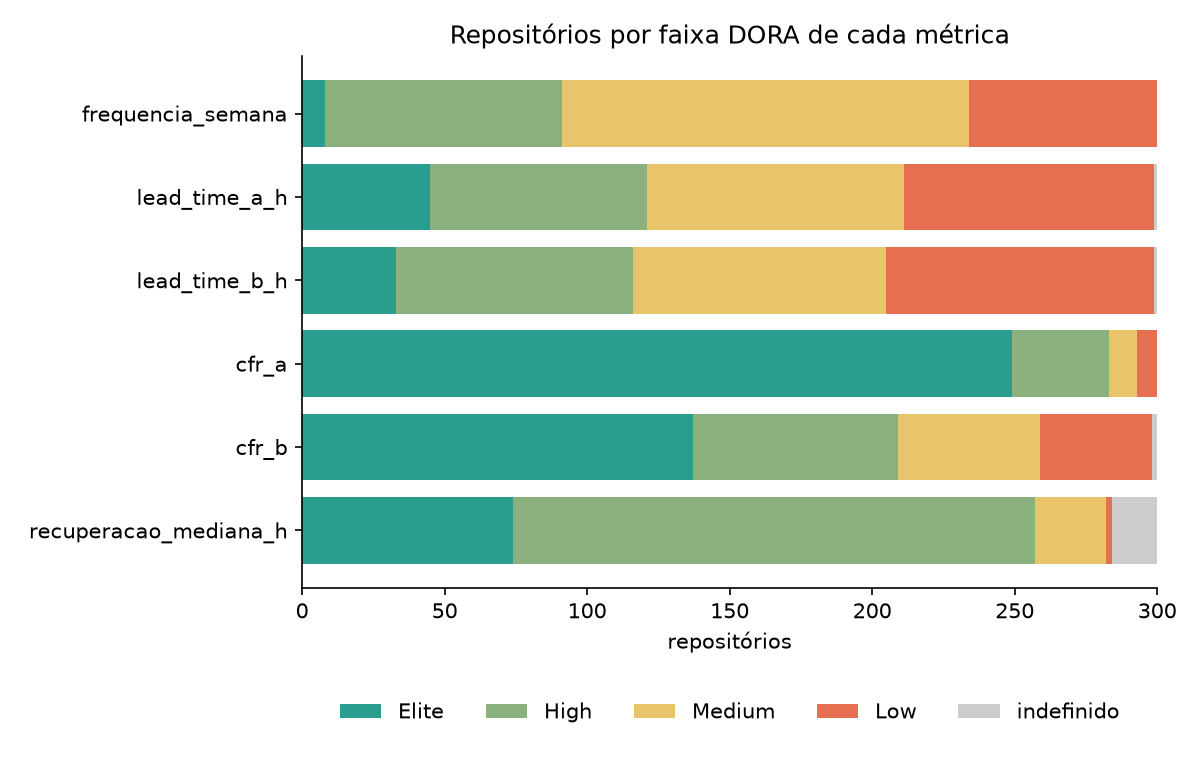
\includegraphics[width=0.75\textwidth]{faixas_por_metrica.png}
\caption{Repositórios por faixa DORA em cada métrica (cinza: métrica indefinida).}
\label{fig:faixas}
\end{figure}

\begin{table}[t]
\centering
\small
\caption{Hipóteses das RQ 01 a RQ 04 frente aos resultados.}
\label{tab:hipoteses}
\begin{tabular}{p{0.04\textwidth}p{0.50\textwidth}p{0.38\textwidth}}
\hline
RQ & Hipótese & Resultado \\
\hline
01 & \textit{Medium} mais comum, \textit{Elite} minoria, \textit{Low} com 5 a 11 releases & Confirmada (\textit{Medium} com 45\%) \\
02 & Dias a poucas semanas, na maioria \textit{Medium} e \textit{High} & Confirmada \\
02 & Variante (a) maior e com mais \textit{Low} que a (b) & Refutada (88 \textit{Low} contra 94) \\
03 & CFR baixo na maioria, com grande dispersão & Confirmada \\
03 & CFR (a) maior que CFR (b) & Refutada (4,7\% contra 17,4\%) \\
04 & Menos de um dia, mediana \textit{High}, com censura & Confirmada \\
04 & Poucos \textit{Elite}, IQR amplo e cauda de dias a semanas & Parcial (26,1\% \textit{Elite}; IQR estreito) \\
\hline
\end{tabular}
\end{table}

\subsection{RQ 01: frequência de deploy}

A faixa \textit{Medium} reúne 135 repositórios (45,0\%), seguida da \textit{High} (83; 27,7\%), da \textit{Low} (74; 24,7\%) e da \textit{Elite} (8; 2,7\%), e o repositório mais frequente publica 49,6 releases por semana, quase cem vezes a mediana. A \textit{Medium} é maioria relativa, e não absoluta. Chama a atenção a cauda lenta: um quarto dos projetos populares publica menos de uma release por mês, o que reforça que estrelas não indicam cadência de entrega.

\subsection{RQ 02: lead time}

O lead time mediano é de 10,7 dias na variante (a) e de 11,5 dias na (b), com distribuições parecidas: na (a), 45 repositórios são \textit{Elite}, 76 \textit{High}, 90 \textit{Medium} e 88 \textit{Low}; na (b), 33, 83, 89 e 94. A variante (a) é maior em 58,9\% dos repositórios, mas por pouco, e a diferença não aparece na distribuição agregada. Uma explicação plausível, não testada, é que a (b) pondera cada commit e dá mais peso às releases grandes, enquanto a (a) dá o mesmo peso a cada release.

\subsection{RQ 03: taxa de falha de mudanças}

No CFR (a), 83,0\% dos repositórios são \textit{Elite}; no CFR (b), 46,0\% são \textit{Elite}, 24,2\% \textit{High}, 16,8\% \textit{Medium} e 13,1\% \textit{Low}. Ao contrário do esperado, a variante (a) é menor em 67,1\% dos repositórios, provavelmente porque divide as falhas por todas as execuções de CI, enquanto a (b) divide por poucas releases (mediana de 28). A (a) mede falha de \textit{pipeline}, e não de produção; a (b) se aproxima mais do DORA, mas depende da heurística de release corretiva (Seção~\ref{sec:validacao}) e deve ser lida como estimativa ruidosa.

\subsection{RQ 04: tempo de recuperação}

Dos 284 repositórios com valor, 90,5\% se recuperam em menos de um dia: 26,1\% são \textit{Elite}, 64,4\% \textit{High}, 8,8\% \textit{Medium} e 0,7\% \textit{Low}. Dezesseis ficam sem valor, por não terem episódio de falha completo, e 0,9\% dos 64\,672 episódios são censurados. A cauda longa esperada não aparece (só 2 repositórios chegam a uma semana, e o IQR é estreito), e os \textit{Elite} são mais de um quarto.
